\subsubsection{Giao diện thông tin cá nhân}
\hspace*{2em} Hình ~\ref{fig:profile} là giao diện hiển thị thông tin cá nhân của người dùng sau khi đăng nhập.  
Tại đây, ứng dụng cung cấp thông tin cơ bản gồm tên, địa chỉ email và ảnh đại diện.  
Nút \textbf{Chỉnh sửa hồ sơ} hiện chỉ mang tính minh họa chưa được triển khai chức năng cập nhật dữ liệu trên hệ thống.  
Người dùng có thể sử dụng nút \textbf{Đăng xuất} để thoát khỏi phiên làm việc.

\begin{figure}[H]
  \centering
  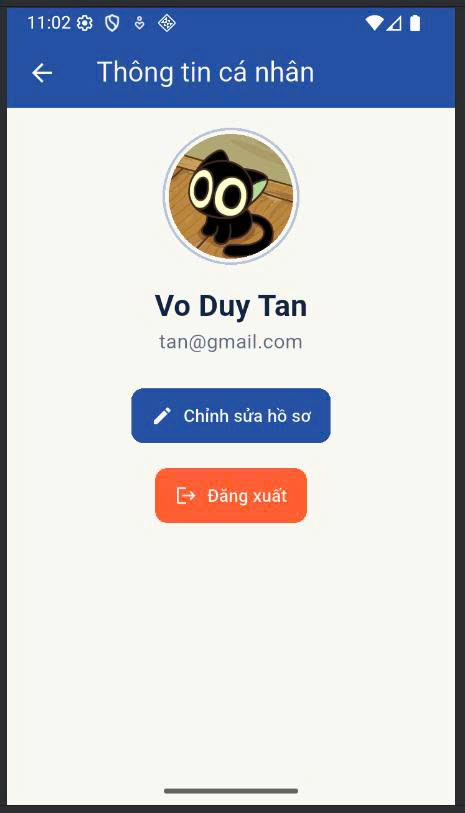
\includegraphics[width=0.5\textwidth]{figures/pic12.jpg}
  \caption{Giao diện hiển thị thông tin cá nhân người dùng.}
  \label{fig:profile}
\end{figure}

\hspace*{2em} Qua các giao diện đã trình bày, có thể thấy ứng dụng được thiết kế với bố cục trực quan, nhất quán và thân thiện với người dùng.  
Từ các màn hình \textbf{Đăng nhập}, \textbf{Đăng ký}, đến giao diện chính với các mục \textbf{Bạn bè}, \textbf{Nhóm} và \textbf{Hội thoại} toàn bộ luồng thao tác được xây dựng rõ ràng giúp người dùng dễ dàng kết nối, trò chuyện và quản lý quan hệ bạn bè.  
Các chức năng như gửi và chấp nhận lời mời kết bạn, trao đổi tin nhắn theo thời gian thực, cũng như quản lý thông tin cá nhân được thể hiện rõ ràng trong từng phần.  
Mặc dù một số tính năng như \textit{Chỉnh sửa hồ sơ} hiện mới dừng ở phần giao diện, chưa hoàn thiện xử lý phía máy chủ nhưng tổng thể hệ thống đã đáp ứng được mục tiêu về \textbf{tính bảo mật, tính ổn định và trải nghiệm sử dụng thân thiện}.  
